\documentclass{article}
\usepackage{graphicx}
\usepackage[margin=1.5cm]{geometry}
\usepackage{amsmath}

\begin{document}

\title{Thursday Reading Assessment: Unit 3, Magnetic Forces and Fields}
\author{Prof. Jordan C. Hanson}

\maketitle

\section{Memory Bank}

\begin{itemize}
\item $\vec{F} = I \vec{L} \times \vec{B}$ ... Lorentz Force on a Current
\item $\vec{F} = q \vec{v} \times \vec{B}$ ... Lorentz Force on a Charge
\item $B = (\mu_0 I)/(2\pi r)$ ... The magnetic field $B$ \textit{caused} by the current $I$ a distance $r$ away.
\end{itemize}

\begin{figure}[ht]
\centering
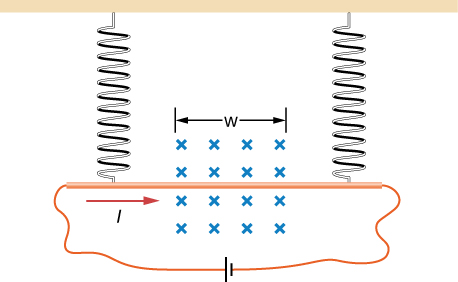
\includegraphics[width=0.25\textwidth]{currentBfieldSpring.jpeg} \hspace{0.2cm}
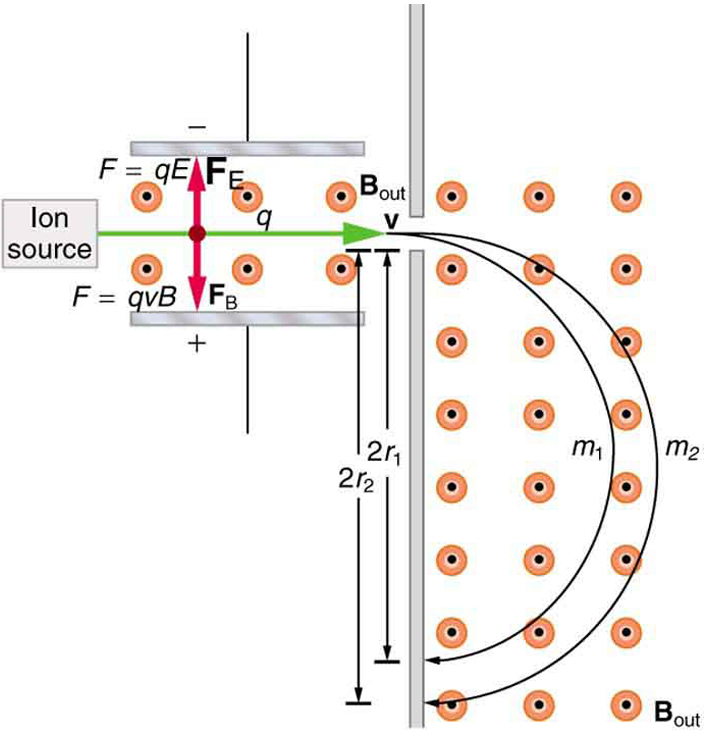
\includegraphics[width=0.2\textwidth]{figures/mass_spec.jpeg} \hspace{0.2cm}
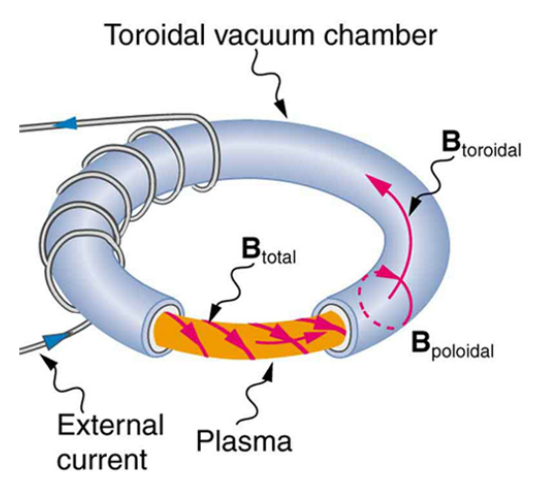
\includegraphics[width=0.3\textwidth]{figures/tokamak.png}
\caption{\label{fig:para} (Left) A current-carrying rod suspended by springs in a B-field.  (Right) Current 1 causes a B-field to exert a Lorentz force on wire 2.  Note that the RHR-2 determines the vector direction of the B-field.}
\end{figure}

\section{Forces on Currents and Charges}

\begin{enumerate}
\item (a) Consider Fig. \ref{fig:para} (left). A metal rod of mass $m$ and length $L$ is hung from the ceiling using two springs of spring constant $k$. A uniform magnetic field of magnitude $B$ pointing perpendicular to the rod and spring exists in a region of space covering a length $w$ of the copper rod.  Determine the change in the length $\Delta y$ of the springs when a current $I$ runs through the copper rod. (b) Consider Fig. \ref{fig:para} (middle). Suppose two ions of equal charge $q$ are launched from the ion source with masses $m_1 = 2 m$ and $m_2 = m$.  In the first stage, the $E$ and $B$-fields are tuned to create $F_{\rm net} = 0$.  Show that the velocity of the ions must be $v = E/B$. (c) In the second stage, $E = 0$ but we have the same $B$-field.  What are the radii $r_1$ and $r_2$, in terms of the given variables? (d) Consider the \textit{tokamak} in Fig. \ref{fig:para} (right).  Using the right-hand rule, convince yourself that the external current creates a $B$-field inside the toroid that runs along the circumference of the toroid.  If there are charged particles moving around the ring, trapped by the toroidal field, use the right-hand rule again to convince yourself these charged particles create a \textit{poloidal} field.
\end{enumerate}

\end{document}
